%===============================================================================
\begin{frame}
\frametitle{Архитектура нейронной сети}
\begin{columns}[T]
    \column{1\textwidth}
    
    \begin{block}{}%{\centering Архитектура НС}
        \vspace{1mm}
        \centering 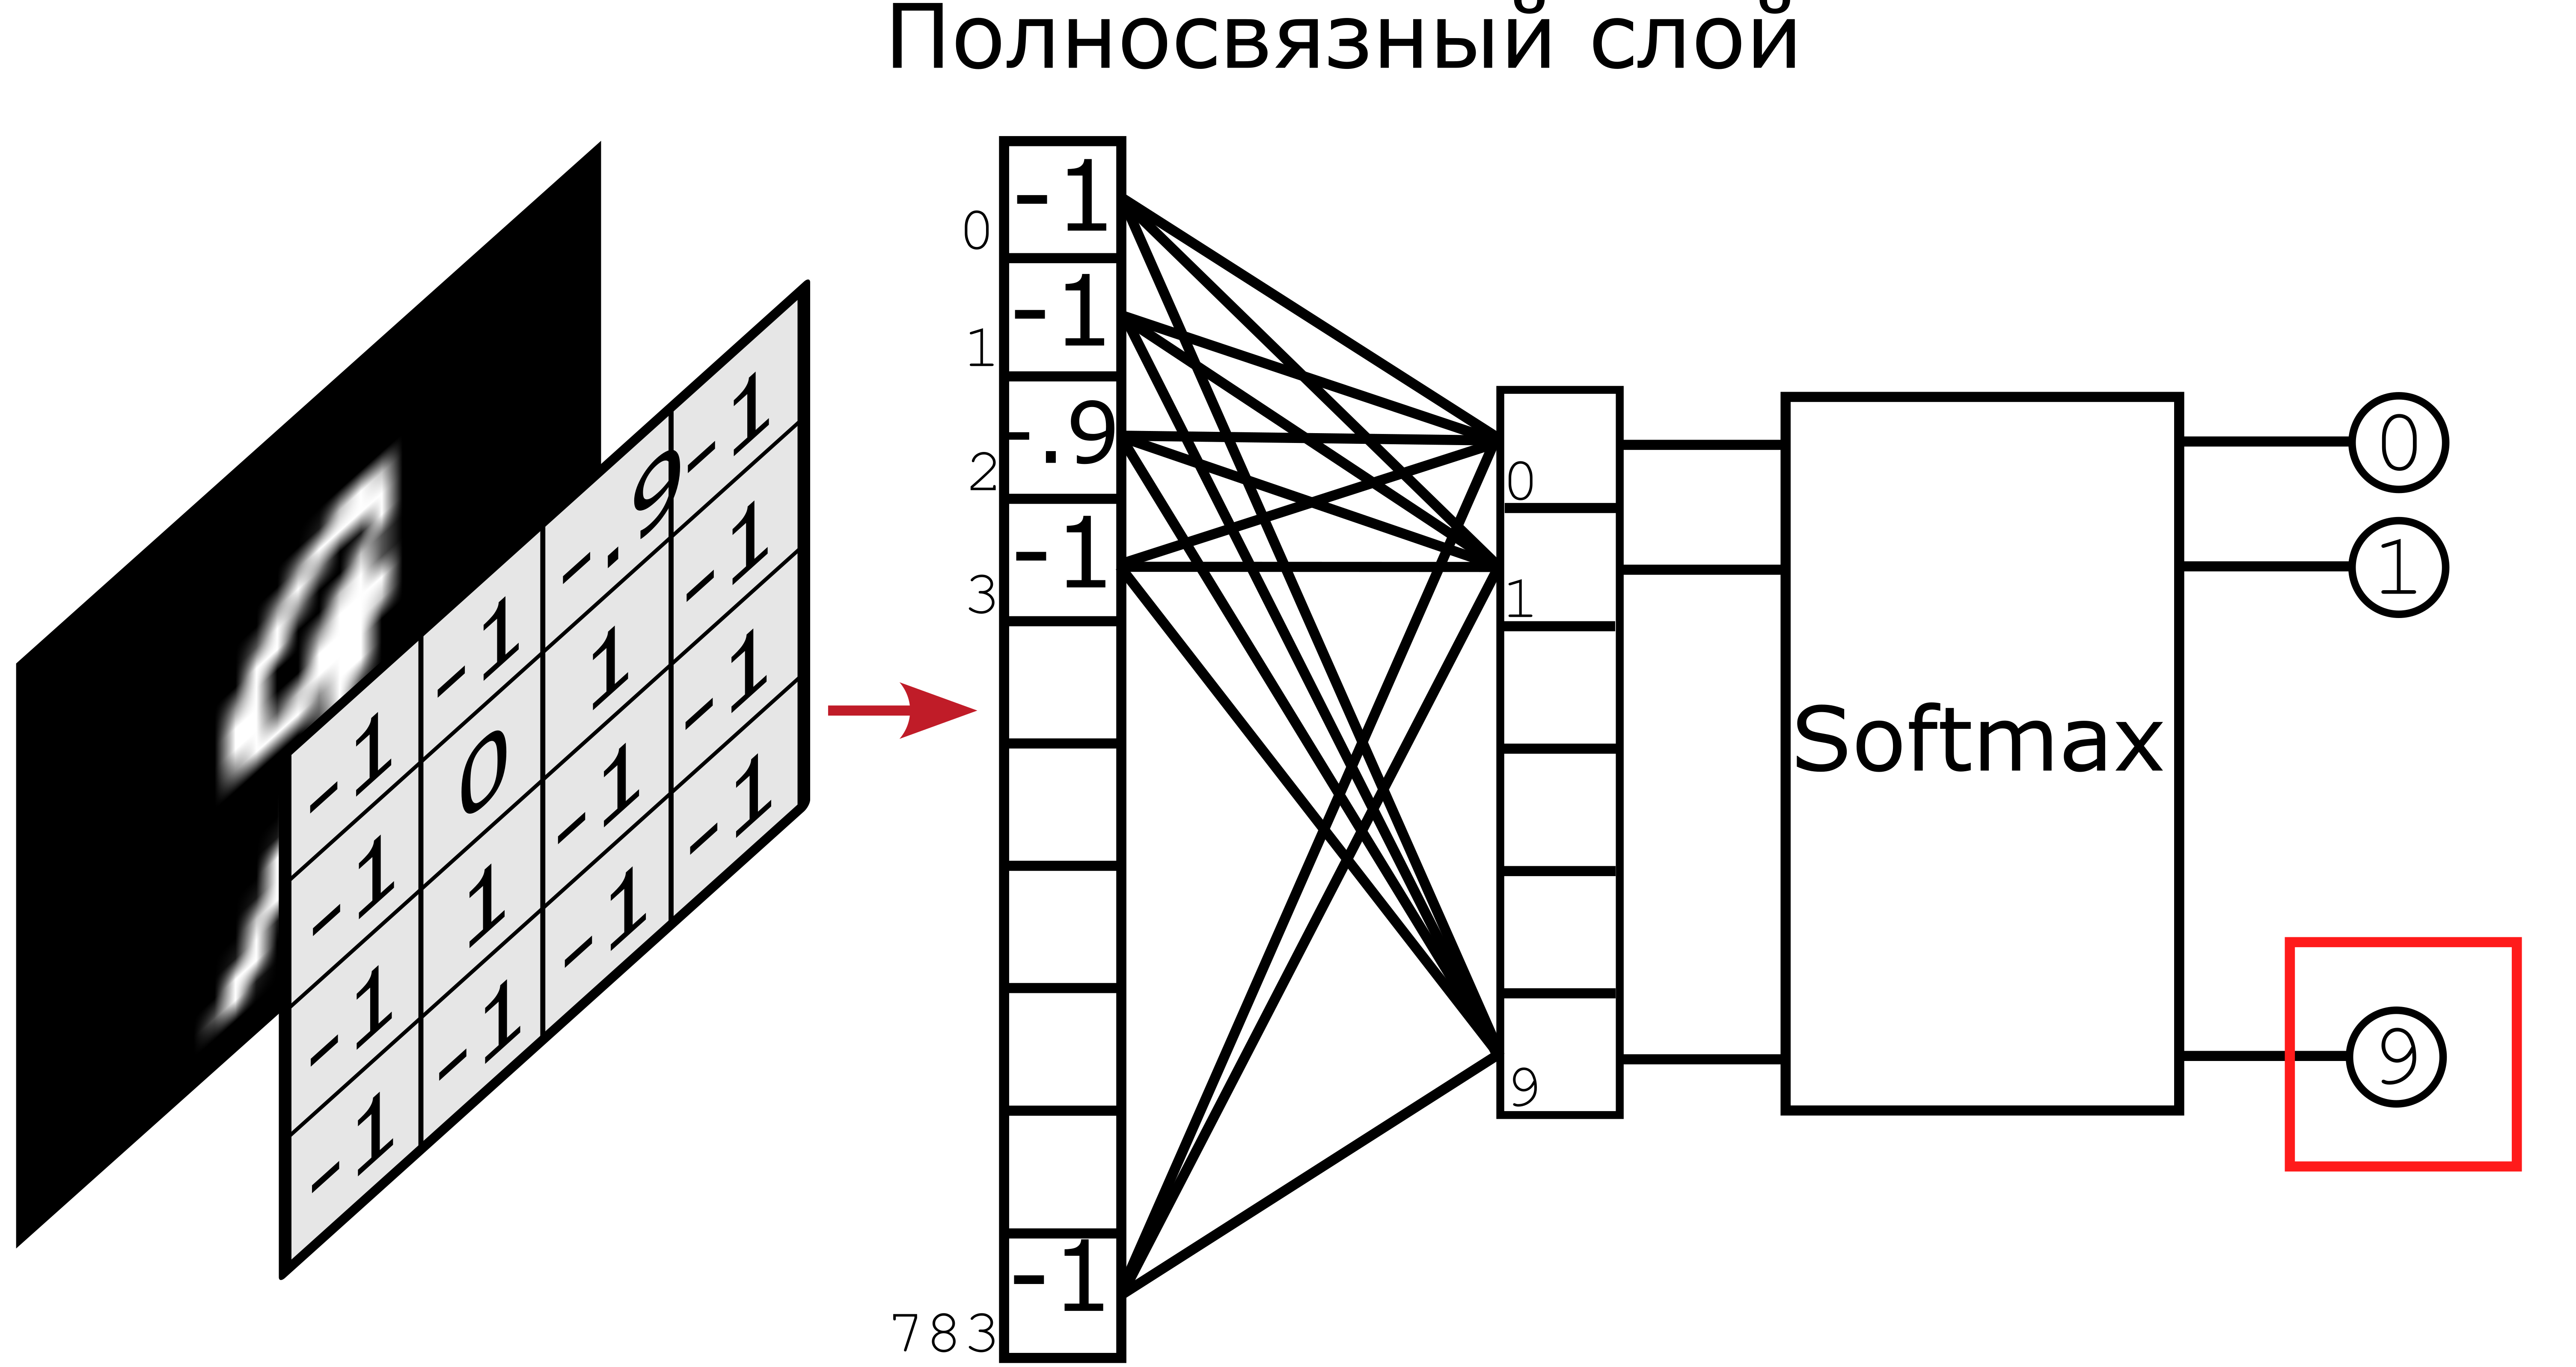
\includegraphics[width = 0.7\textwidth]{pics/nn_2.png}
        % \includesvg[height = 0.4\textheight]{basic_AE.svg}        
    \end{block}        

    \column{1\textwidth}
    \vspace{-2mm}
        
\end{columns}
\end{frame}
%===============================================================================
\begin{frame}[t]
    \frametitle{Параметры для обучения}
    \begin{columns}[T]
    \column[t]{0.5\textwidth}
    \begin{block}{\centering Параметры обучения}                
        \begin{itemize}\small
            \item Входные данные приводятся к диапазону [-1, 1] и устанавливается их
            среднеквадратическое отклонение(СКО) равным 0,5
            \item Оптимизация производилась с использованием метода стохастического градиентного спуска (SGD)
            (скорость обучения $\eta =3 \cdot 10^{-3}$, число эпох -- 10000, моментум $\gamma = 0,9$)
        \end{itemize}
    \end{block}
     
    \column[t]{0.5\textwidth}
    \begin{block}{\centering График функции потерь}
        \vspace{3mm}
        \centering 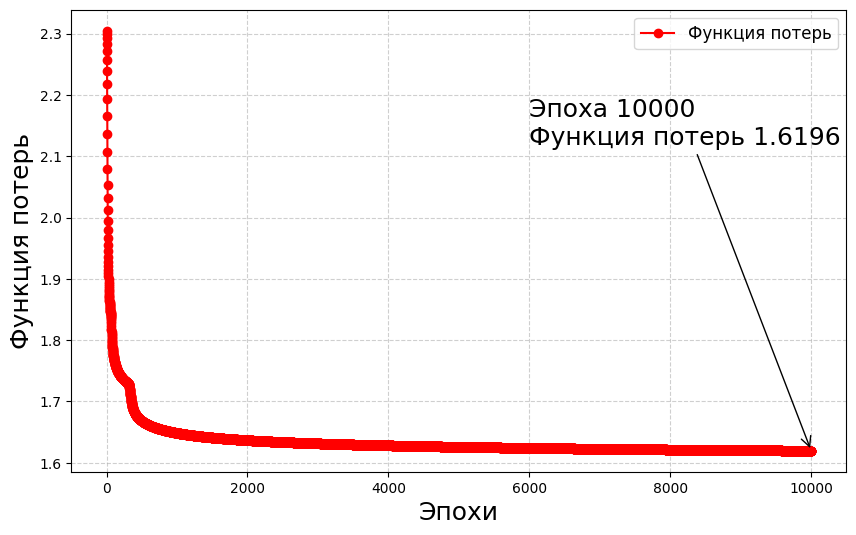
\includegraphics[width = 0.9\textwidth]{pics/loss.png} 
    \end{block}
    \end{columns}
    % \begin{itemize}
    %     \item Входные данные приводятся к диапазону [-1, 1] и устанавливается их
    %     среднеквадратическое отклонение(СКО) равным 0,5
    %     \item Оптимизация производилась с использованием метода стохастического градиентного спуска (SGD)
    %     (скорость обучения $\eta =3 \cdot 10^{-3}$, число эпох -- 10000, моментум $\gamma = 0,9$)
    % \end{itemize}
    
    \end{frame}
    